\documentclass[10.5pt]{article}

% ---------- Page geometry ----------
\usepackage[a4paper, margin=2.1cm, top=2.3cm, bottom=2.4cm]{geometry}
\usepackage[utf8]{inputenc}
\usepackage[T1]{fontenc}

% ---------- Core packages ----------
\usepackage{titlesec}
\usepackage{enumitem}
\usepackage{fancyhdr}
\usepackage{xcolor}
\usepackage{tikz}
\usetikzlibrary{shapes.geometric, arrows.meta, positioning, fit, backgrounds, calc}
\usepackage{booktabs}
\usepackage{array}
\usepackage{longtable}
\usepackage{colortbl}
\usepackage{graphicx}
\usepackage{amsmath, amssymb}
\usepackage{tcolorbox}
\tcbuselibrary{skins, breakable}
\usepackage{hyperref}
\usepackage{multicol}
\usepackage{ragged2e}

% ---------- Colours ----------
\definecolor{isroblue}{HTML}{0B2340}
\definecolor{accent}{HTML}{1D6FB8}
\definecolor{accent2}{HTML}{E8672A}
\definecolor{winbadge}{HTML}{1E7F52}
\definecolor{lightbg}{HTML}{F4F7FB}
\definecolor{tablehead}{HTML}{0B2340}
\definecolor{softgray}{HTML}{666666}
\definecolor{ruleline}{HTML}{D6DEE8}

\hypersetup{
    colorlinks=true,
    linkcolor=accent,
    urlcolor=accent,
    citecolor=accent,
    pdftitle={Intelligent Dead Reckoning System - Technical Proposal},
    pdfauthor={SIH Team},
    pdfsubject={AI-ML based Intelligent Dead Reckoning system for seamless navigation},
}

% ---------- Section styling ----------
\titleformat{\section}
  {\Large\bfseries\color{isroblue}}
  {\thesection}{0.4em}{}[{\color{ruleline}\titlerule[1pt]}]
\titlespacing*{\section}{0pt}{1.4em}{0.8em}

\titleformat{\subsection}
  {\large\bfseries\color{accent}}
  {\thesubsection}{0.4em}{}
\titlespacing*{\subsection}{0pt}{1.1em}{0.5em}

\titleformat{\subsubsection}
  {\normalsize\bfseries\color{isroblue}}
  {\thesubsubsection}{0.4em}{}
\titlespacing*{\subsubsection}{0pt}{0.9em}{0.4em}

% ---------- Header / footer ----------
\pagestyle{fancy}
\setlength{\headheight}{20pt}
\fancyhf{}
\renewcommand{\headrulewidth}{0.4pt}
\renewcommand{\headrule}{\hbox to\headwidth{\color{ruleline}\leaders\hrule height \headrulewidth\hfill}}
\fancyhead[L]{\small\color{softgray} Intelligent Dead Reckoning System -- Technical Proposal}
\fancyhead[R]{\small\color{softgray} SIH Problem Statement 26168}
\fancyfoot[C]{\small\color{softgray}\thepage}

% ---------- Custom boxes ----------
\newtcolorbox{keyinsight}[1][]{
  enhanced, breakable, colback=lightbg, colframe=accent,
  boxrule=0.6pt, left=8pt, right=8pt, top=6pt, bottom=6pt,
  arc=1.5pt,
  title={\textbf{\small #1}},
  fonttitle=\color{isroblue},
  coltitle=isroblue,
  attach boxed title to top left={xshift=8pt, yshift=-2.2mm},
  boxed title style={colback=lightbg, boxrule=0pt},
  before skip=8pt, after skip=8pt
}

\newtcolorbox{winbox}[1][]{
  enhanced, breakable, colback=winbadge!6, colframe=winbadge,
  boxrule=0.7pt, left=8pt, right=8pt, top=6pt, bottom=6pt, arc=1.5pt,
  title={\textbf{\small \textcolor{white}{#1}}},
  colbacktitle=winbadge,
  before skip=8pt, after skip=8pt
}

\newtcolorbox{diffbox}[1][]{
  enhanced, breakable, colback=accent2!5, colframe=accent2,
  boxrule=0.7pt, left=8pt, right=8pt, top=6pt, bottom=6pt, arc=1.5pt,
  title={\textbf{\small \textcolor{white}{#1}}},
  colbacktitle=accent2,
  before skip=8pt, after skip=8pt
}

% ---------- Misc ----------
\renewcommand{\arraystretch}{1.25}
\setlist[itemize]{leftmargin=1.4em, itemsep=2pt, topsep=3pt}
\setlist[enumerate]{leftmargin=1.6em, itemsep=2pt, topsep=3pt}

\newcommand{\tstack}[1]{\textcolor{accent}{\textbf{#1}}}

%=================================================================
\begin{document}

% ================= TITLE PAGE =================
\begin{titlepage}
\newgeometry{margin=2.2cm}
\begin{center}
\vspace*{0.6cm}

{\small\color{softgray} SMART INDIA HACKATHON $\cdot$ PROBLEM STATEMENT ID 26168}\\[0.3cm]
{\color{ruleline}\rule{\linewidth}{0.6pt}}\\[1.0cm]

{\Huge\bfseries\color{isroblue} AI/ML--Based Intelligent Dead\\[0.2cm] Reckoning for Seamless Navigation}\\[0.8cm]

{\Large\color{accent}\textbf{Technical Architecture, Differentiation \&}}\\[0.15cm]
{\Large\color{accent}\textbf{High-Level Implementation Design}}\\[1.4cm]

\begin{tikzpicture}
\node[draw=accent, fill=lightbg, rounded corners=2pt, line width=0.6pt,
      text width=13.5cm, align=left, inner sep=12pt] {
  \small
  \textbf{\color{isroblue}Organisation:} Indian Space Research Organisation (ISRO) \\
  \textbf{\color{isroblue}Department:} Department of Space \\
  \textbf{\color{isroblue}Category:} Software \quad $\vert$ \quad \textbf{\color{isroblue}Theme:} Smart Vehicles \\
  \textbf{\color{isroblue}Benchmark dataset:} IO-VNBD -- Inertial \& Odometry Vehicle Navigation \\
  \hspace{2.05cm} Benchmark Dataset (Onyekpe et al., Coventry University)
};
\end{tikzpicture}

\vspace{1.6cm}

{\color{ruleline}\rule{0.5\linewidth}{0.4pt}}\\[0.5cm]
{\large\color{softgray} Proposal prepared for the Bharatiya Antariksh Hackathon / SIH finale submission}\\[0.2cm]
{\small\color{softgray} This document details the proposed system architecture, technology stack,\\
the specific technical differentiators of our approach relative to the standard\\
literature pipeline, and a high-level design for implementation.}

\end{center}
\vfill
\restoregeometry
\end{titlepage}

\tableofcontents
\thispagestyle{empty}
\newpage

% ================= SECTION 1 =================
\section{Problem Restatement and Core Challenge}

Smartphone-based navigation is the \emph{de facto} positioning layer for the overwhelming majority of Indian road users -- commercial trucks, older cars without factory INS, and, critically, the tens of millions of two-wheelers that dominate Indian traffic. None of these have an OBD-II-fed wheel-speed reference available to a navigation app. When GNSS drops -- tunnels, underpasses, multi-level parking, dense urban canyons, forested highways -- these apps are left with nothing but a consumer-grade MEMS IMU riding in a phone mount that is itself vibrating, sliding, and shaking on the vehicle chassis.

\begin{keyinsight}[The real problem is not ``do dead reckoning'' -- it is ``dead reckoning without integration blowing up''.]
Classical strapdown INS mechanization double-integrates noisy accelerometer output. Bias, scale-factor error, and misalignment enter the position estimate as a \emph{quadratic}-in-time error term. On a MEMS-grade smartphone IMU this alone is enough to put you off the road within seconds of GNSS loss -- long before ISRO's benchmark window of 50\,m drift in 1 minute or 100\,m over 1\,km at 60\,km/h has elapsed. Any solution that is fundamentally ``integrate, then correct'' is fighting this quadratic term for its entire life. Our architecture is built around \emph{breaking that dependency}, not just slowing it down.
\end{keyinsight}

\subsection{What the Problem Statement Explicitly Requires}
\begin{itemize}
\item An in-vehicle alignment/calibration engine (pitch, roll, yaw relative to driving direction) working for both dashboard mounts and holders.
\item An AI speed \& vibration filter that estimates forward velocity directly from noisy IMU signals -- \textbf{no OBD-II, no external speedometer}.
\item Map-matching with non-holonomic constraints against an offline OSM database.
\item A GNSS+INS AI fusion engine that mitigates drift and hands off seamlessly, in both directions, within milliseconds.
\item A deliverable that is \emph{both} a mobile app (phone IMU) \emph{and} a portable edge-deployable engine (any external IMU, including FOG-grade sensors at $\sim$200\,Hz).
\item Hard benchmark: $<$10\% positional drift during blackout (e.g. $<$5\,m over 50\,m/1\,min, or $<$100\,m over 1\,km at 60\,km/h); 10\,Hz fused position update on phone, higher on the edge engine.
\end{itemize}

% ================= SECTION 2 =================
\section{Why the ``Obvious'' Solution Caps Out}

Given the problem statement's own wording (LSTM/TCN bias correction $\rightarrow$ EKF/UKF fusion $\rightarrow$ NHC $\rightarrow$ HMM map-matching), the large majority of competing teams will converge on the same architecture:

\begin{center}
\begin{tikzpicture}[
  node distance=0.55cm and 0.55cm,
  box/.style={draw=softgray, fill=white, rounded corners=1.5pt, minimum height=0.85cm, text width=2.55cm, align=center, font=\scriptsize, line width=0.5pt},
  arrow/.style={-{Stealth[length=2mm]}, softgray, line width=0.6pt}
]
\node[box] (a) {Raw IMU\\stream};
\node[box, right=of a] (b) {LSTM/TCN\\bias correction};
\node[box, right=of b] (c) {Integrate\\to velocity/pos.};
\node[box, right=of c] (d) {EKF / UKF\\+ NHC};
\node[box, right=of d] (e) {HMM\\map-matching};
\draw[arrow] (a) -- (b);
\draw[arrow] (b) -- (c);
\draw[arrow] (c) -- (d);
\draw[arrow] (d) -- (e);
\end{tikzpicture}
\end{center}

\vspace{-0.2cm}
This pipeline is legitimate and will pass a basic screening, but it inherits a structural weakness: \textbf{the trajectory is still produced by integration.} Learned bias correction reduces the constant of proportionality on the drift term; it does not remove the quadratic growth. Three further gaps are common across this class of solution, all of which map directly onto ISRO's stated requirements:

\begin{enumerate}
\item \textbf{Single point of failure in velocity estimation.} One IMU-derived speed estimate feeds the whole chain. If the gyro-based orientation is briefly wrong (a pothole, the phone sliding in its holder), there is no independent channel to catch it.
\item \textbf{One model, one vehicle.} Models are trained and demoed on a single test vehicle. The PS explicitly targets ``commercial trucks, older cars, and millions of two-wheelers'' -- a diesel truck's chassis vibration signature, a scooter's, and a sedan's are not remotely the same distribution, and a model that is not \emph{recalibrated} per vehicle will silently degrade off-stage.
\item \textbf{Drift is corrected, never bounded.} Kalman-style fusion pulls the estimate back toward plausibility but has no external anchor during a long blackout; over a 1\,km tunnel at 60\,km/h, the correction has to work perfectly for the full 60 seconds with zero absolute reference.
\end{enumerate}

% ================= SECTION 3 =================
\section{Our Architecture -- System Overview}

We keep the components ISRO explicitly asked for (alignment engine, AI speed filter, NHC map-matching, GNSS+INS fusion, seamless handoff) but change \emph{what corrects the trajectory} and \emph{how many independent evidence sources feed the fusion step}. The architecture adds two new subsystems that do not exist in the standard pipeline: a \textbf{Road-Signature Drift-Anchor} and a \textbf{Dual-Channel Velocity Estimator}, plus a per-vehicle \textbf{on-device calibration pass} that the standard pipeline treats as out of scope.

\begin{center}
\begin{tikzpicture}[
  node distance=6mm and 6mm,
  stage/.style={draw=isroblue, fill=lightbg, rounded corners=2pt, line width=0.6pt, text width=3.05cm, minimum height=1.05cm, align=center, font=\scriptsize},
  hl/.style={draw=accent2, fill=accent2!8, rounded corners=2pt, line width=0.9pt, text width=3.05cm, minimum height=1.05cm, align=center, font=\scriptsize},
  lbl/.style={font=\scriptsize\bfseries, color=softgray},
  arr/.style={-{Stealth[length=2mm]}, isroblue, line width=0.6pt},
  arrhl/.style={-{Stealth[length=2mm]}, accent2, line width=0.9pt}
]

% Row 1: sensors
\node[stage] (imu) {Phone IMU\\(acc + gyro + mag)};
\node[stage, right=of imu] (gnss) {GNSS receiver\\(intermittent)};
\node[stage, right=of gnss] (map) {Offline OSM\\road graph};

% Row 2: alignment + dual velocity
\node[stage, below=10mm of imu] (align) {Alignment \& mount\\calibration engine};
\node[hl, below=10mm of gnss] (velA) {Channel A:\\NHC-constrained\\learned-bias velocity};
\node[hl, right=6mm of velA] (velB) {Channel B:\\accelerometer-only\\velocity net};

% Row 3: fusion + anchor
\node[hl, below=13mm of velA] (fuse) {AI GNSS+INS\\Fusion Engine\\(UKF core)};
\node[hl, right=6mm of fuse] (anchor) {Road-Signature\\Drift-Anchor\\(segment classifier)};

% Row 4: output
\node[stage, below=13mm of fuse] (mm) {HMM Map-Matching};
\node[stage, right=6mm of mm] (out) {Fused position\\@10Hz (phone) /\\200Hz (edge)};

\draw[arr] (imu) -- (align);
\draw[arr] (align) -- (velA);
\draw[arr] (imu.south) to[out=-90,in=90] (velB.north);
\draw[arrhl] (velA) -- (fuse);
\draw[arrhl] (velB) -- (fuse);
\draw[arr] (gnss) -- (fuse);
\draw[arrhl] (imu.east) to[out=0,in=90] (anchor.north);
\draw[arrhl] (map) to[out=-90,in=90] (anchor.north east);
\draw[arrhl] (anchor) -- (fuse);
\draw[arr] (fuse) -- (mm);
\draw[arr] (map.south) to[out=-90,in=90] (mm.north east);
\draw[arr] (mm) -- (out);

\end{tikzpicture}
\end{center}

\begin{center}
{\scriptsize \textcolor{accent2}{$\blacksquare$} orange = subsystems absent from the standard literature pipeline (Section 2) \quad
\textcolor{isroblue}{$\blacksquare$} navy = components explicitly required by the PS}
\end{center}

\subsection{Component Responsibilities}
\begin{itemize}
\item \textbf{Alignment \& Mount Calibration Engine} -- estimates pitch/roll/yaw of the phone relative to the vehicle's direction of travel from gravity-vector tracking plus a learned mounting-angle regressor (MountNet-style), refreshed continuously so a knocked or re-seated phone re-aligns within seconds, not after a full re-install.
\item \textbf{Channel A (NHC-constrained learned-bias velocity)} -- an LSTM/TCN corrects accelerometer/gyro bias and scale error; the corrected signal is integrated under non-holonomic constraints (no lateral slip, no vertical fly-off) to produce a forward-velocity estimate. This is the ``expected'' channel.
\item \textbf{Channel B (accelerometer-only velocity net)} -- a lightweight 1D-CNN regresses forward speed directly from a rolling window of raw accelerometer data alone, with no dependency on gyro-derived orientation. It cannot itself replace Channel A's accuracy, but it shares none of Channel A's failure modes (misalignment error, gyro drift, orientation singularities), so it is the cheapest possible independent cross-check available on commodity hardware.
\item \textbf{Road-Signature Drift-Anchor} -- classifies which pre-mapped road segment the vehicle is currently on from its vibration signature, and periodically re-centres the fused position estimate on that segment's midpoint, bounding otherwise-unbounded integration drift.
\item \textbf{AI GNSS+INS Fusion Engine} -- a UKF whose innovation vector now has \emph{four} evidence sources instead of the usual two (GNSS when available, Channel A velocity, Channel B velocity, and the road-segment anchor), with a learned, context-dependent weighting of each source's trust.
\item \textbf{HMM Map-Matching} -- final snap of the fused trajectory onto the OSM road graph, standard Viterbi-style HMM over candidate road edges.
\end{itemize}

% ================= SECTION 4 =================
\section{Technology Stack}

\subsection{Layer-by-Layer Breakdown}

\begin{longtable}{@{}p{2.7cm}p{4.6cm}p{7.4cm}@{}}
\toprule
\rowcolor{tablehead}
\textcolor{white}{\textbf{Layer}} & \textcolor{white}{\textbf{Technology}} & \textcolor{white}{\textbf{Why this choice}} \\
\midrule
\endhead
\textbf{Model training} (cloud/desktop) & PyTorch, PyTorch Lightning, Weights \& Biases for experiment tracking & Fast iteration on IO-VNBD + collected data; native ONNX export path for on-device deployment. \\
\textbf{Model export / edge runtime} & ONNX Runtime Mobile, TensorFlow Lite (post-training int8 quantisation), Core ML (iOS path) & Sub-10\,ms inference for a $\sim$100k-parameter TCN/CNN on a mid-range Android SoC; quantisation keeps the full stack under $\sim$5-8\,MB on-device. \\
\textbf{Mobile application} & Android: Kotlin + Jetpack Compose; sensor access via Android \texttt{SensorManager} at max native rate ($\ge$100\,Hz); background service with foreground notification for continuous logging & Native sensor access is required for the raw, unfiltered accelerometer/gyro stream -- Android's own fused ``linear acceleration'' virtual sensor is \emph{not} used, since it already applies an opaque low-pass/gravity-removal pipeline that would compete with our own learned filters. \\
\textbf{On-device signal processing} & Custom Kotlin/C++ (NDK) ring-buffer + FIR pre-filter, executed before every model call & Keeps the hot path (100+\,Hz sensor callback) off the JVM heap and GC-safe. \\
\textbf{Sensor fusion core} & Custom Unscented Kalman Filter (Python for prototyping $\to$ C++ for production), state vector $[p_n, p_e, v_n, v_e, \psi, b_a, b_g]$ & UKF over EKF because the heading/velocity coupling under hard cornering and roundabouts (both explicitly present in IO-VNBD) is mildly non-linear; UKF's sigma-point propagation handles this without a Jacobian. \\
\textbf{Map-matching} & Offline OSM extract (via Osmium / \texttt{osmnx} at build time) + custom HMM/Viterbi decoder, GraphHopper-style routing graph for road-segment adjacency & Fully offline -- no live map API calls, matching the PS's ``offline map database'' requirement and keeping the app usable in exactly the zero-connectivity scenarios it targets. \\
\textbf{Road-signature module} & 1D-CNN classifier (3 conv blocks, mean-pool) trained per-region on GNSS-labelled drive data; SQLite/Room on-device store of segment signatures & Small enough to ship per-city/per-corridor signature packs (a few MB each) rather than one global model, matching how road surfaces actually vary across India. \\
\textbf{Per-vehicle calibration} & On-device transfer-learning adapter (last-layer / LoRA-style fine-tune, $<$50k trainable parameters) triggered during a short GNSS-available calibration drive & Keeps the recalibration pass fast enough (10--30\,s) and light enough to run entirely on-phone, with no server round-trip. \\
\textbf{Edge-deployable engine (non-phone)} & Same PyTorch models cross-compiled via ONNX Runtime C++ API; reference target -- Raspberry Pi CM4 / Jetson Orin Nano class board reading a FOG-grade IMU over UART/SPI at $\sim$200\,Hz & Identical model weights and fusion core as the phone app -- the ``mobile app'' and ``edge engine'' deliverables share one codebase, differing only in the sensor-ingest and I/O adapters, directly satisfying the PS's ``not constricted to smartphone IMU alone'' requirement. \\
\textbf{Data / dataset tooling} & IO-VNBD (Coventry Univ.) as primary benchmark; Python (\texttt{pandas}, \texttt{numpy}, \texttt{scipy}) for the synchronisation \& windowing pipeline & IO-VNBD ships both vehicle-extracted and smartphone-recorded, synchronised and unsynchronised, sensor streams -- exactly matching our dual-channel training requirement. \\
\textbf{UI / navigation surface} & Mapbox Navigation SDK (offline tile mode) or a custom MapLibre GL layer over the OSM extract & Smooth vehicle-icon rendering and route rendering without a live-tile dependency, satisfying the ``uninterrupted vehicle icon'' requirement even fully offline. \\
\bottomrule
\end{longtable}

\subsection{Why We Avoid a Few Common Choices}
\begin{itemize}
\item \textbf{No Android fused ``linear acceleration'' sensor as primary input.} It silently mixes in a vendor-specific gravity/orientation filter we cannot audit or retrain; we take raw accelerometer + gyro + magnetometer and own the entire filtering chain.
\item \textbf{No cloud inference in the critical loop.} Every model that touches the live trajectory (alignment, both velocity channels, fusion, road-signature classification) runs on-device. Cloud is used only for offline training and for periodically shipping updated per-region road-signature packs -- never for a real-time call, since a tunnel by definition has no connectivity to call out to.
\item \textbf{No single monolithic model.} Splitting alignment / Channel A / Channel B / road-signature into separate small models (each well under 1\,MB quantised) is deliberately chosen over one large end-to-end network: it keeps each failure mode isolated and independently testable, and lets the fusion engine reason about \emph{per-source} trust rather than trusting one black box completely.
\end{itemize}

\newpage
% ================= SECTION 5 =================
\section{Core Technical Differentiators}

\begin{diffbox}[THE THREE PILLARS THAT SEPARATE THIS FROM A STANDARD SUBMISSION]
1. Road-Signature Drift-Anchor -- bounds drift instead of only slowing it. \\
2. Dual-Channel, Failure-Independent Velocity Estimation -- a free consistency check nobody else builds. \\
3. On-Device Per-Vehicle Transfer Calibration -- the only approach that actually survives India's real vehicle mix.
\end{diffbox}

\subsection{Pillar 1 -- Road-Signature Drift-Anchor}
Every vehicle's suspension, tyre, and chassis respond to a given stretch of road surface with a repeatable vibration signature. We exploit this as an \emph{absolute, GNSS-independent} positional anchor rather than as noise to be filtered away.

\textbf{How it works.} During normal GNSS-available driving, the app silently logs (IMU window, GNSS-tagged road segment) pairs for the corridors a user regularly drives. A compact 1D-CNN is trained to classify a 2-second IMU window into one of $N$ fixed-length segments along a known route/corridor. During a blackout, this classifier runs continuously in parallel with the main fusion loop; whenever it reports high-confidence agreement with the fused trajectory's current segment, the position estimate is \emph{re-centred} on that segment's midpoint, resetting the accumulated integration error to at most half a segment length rather than letting it grow for the full blackout duration.

\begin{keyinsight}[Why this specifically wins on ISRO's benchmark]
The benchmark is stated as \emph{drift as a percentage of distance travelled}, not as a function of time. A pure Kalman/NHC pipeline's error still grows roughly with elapsed blackout time. A periodic segment-reset makes worst-case error a function of \emph{segment length}, not of tunnel length -- so a 5\,km tunnel is not structurally harder than a 500\,m one, which a pure-integration competitor cannot claim.
\end{keyinsight}

\textbf{Where the segments come from.} Segment boundaries and signature packs are pre-computed offline per corridor from the same OSM extract already required for map-matching, so this adds no new infrastructure requirement -- it reuses data the PS already mandates the system to carry.

\subsection{Pillar 2 -- Dual-Channel, Failure-Independent Velocity Estimation}
Channel A (bias-corrected, NHC-integrated) and Channel B (accelerometer-only, orientation-independent) are trained to solve the \emph{same} problem through structurally different failure modes:

\begin{center}
\begin{tabular}{@{}p{4.6cm}p{5.6cm}p{4.6cm}@{}}
\toprule
\rowcolor{tablehead}
\textcolor{white}{\textbf{}} & \textcolor{white}{\textbf{Channel A (primary)}} & \textcolor{white}{\textbf{Channel B (cross-check)}} \\
\midrule
Inputs & Bias-corrected acc.\ + gyro, integrated under NHC & Raw accelerometer window only \\
Fails when & Gyro/orientation is briefly wrong (pothole shock, phone slip) & Sustained, wrongly, only under near-constant-vibration edge cases \\
Cost & Higher accuracy, higher compute & Cheap, low-latency, always-on sanity check \\
\bottomrule
\end{tabular}
\end{center}

\textbf{Fusion logic.} The UKF's innovation weighting includes an agreement term between Channel A and Channel B. When they diverge beyond a learned threshold, the fusion engine automatically down-weights Channel A for that epoch and leans on Channel B plus the road-signature anchor -- catching exactly the failure class (mount slip, pothole-induced gyro glitch) that a single-channel pipeline has no way to detect, let alone correct, in real time.

\subsection{Pillar 3 -- On-Device Per-Vehicle Transfer Calibration}
This is the pillar most directly tied to what ISRO is actually asking for and to what most competing teams will skip, because it is unglamorous relative to model architecture work.

\begin{keyinsight}[The PS explicitly targets a vehicle-heterogeneous fleet]
``\emph{...commercial trucks, older cars, and millions of two-wheelers...}'' A model trained once on a single demo vehicle will not transfer cleanly to a completely different suspension, chassis mass, and vibration spectrum -- a truck, an auto-rickshaw, and a Royal Enfield do not share a vibration distribution.
\end{keyinsight}

\textbf{Implementation.} On first use with a given vehicle, the app runs a short (10--30 second) guided calibration drive while GNSS is still available. A small adapter block (last-layer fine-tune, LoRA-style, under 50k trainable parameters) is refit against that vehicle's own accelerometer/gyro statistics and the phone's specific mount, using GNSS-derived ground truth as the label. This adapter is cached per vehicle profile, so switching between a personal scooter and a rented car simply means switching calibration profiles, not retraining from scratch.

\subsection{Comparative Positioning Against Published Approaches}

\begin{longtable}{@{}p{3.1cm}p{3.1cm}p{4.3cm}p{4.9cm}@{}}
\toprule
\rowcolor{tablehead}
\textcolor{white}{\textbf{Approach}} & \textcolor{white}{\textbf{Core idea}} & \textcolor{white}{\textbf{Limitation for this PS}} & \textcolor{white}{\textbf{How our system improves on it}} \\
\midrule
\endhead
WhONet / R-WhONet (Onyekpe et al.) & LSTM learns wheel-encoder error for correction & Requires a physical wheel encoder -- unavailable on two-wheelers and most aftermarket phone setups & We keep R-WhONet's \emph{transfer-learning recalibration idea} but apply it to phone-IMU-only Channel A, with no wheel-encoder dependency \\
OdoNet / DeepOdo & CNN/CNN-GRU pseudo-odometer from IMU (+ barometer), used purely as an NHC-alternative speed aid & Single-channel; failure of the underlying IMU orientation estimate silently degrades the whole pseudo-odometer & Channel B is built as an \emph{independent}, orientation-free channel specifically to catch this failure mode, not as the only speed source \\
CarSpeedNet (Or et al.) & Speed regression from accelerometer only, no gyro/wheel data at inference & Used stand-alone; does not itself solve positional drift or map-matching & Adopted as Channel B \emph{inside} a larger fusion loop, paired with the road-signature anchor for actual position, not just speed \\
Road-vibration road-segmentation (Or, Freydin et al.) & Classify current road segment from vibration signature; report segment midpoint as position & Positioning \emph{is} the segment midpoint -- coarse by itself, and never combined with continuous INS for fine-grained trajectory shape & Used as a periodic \emph{drift-reset anchor} inside a continuous UKF, not as the sole position output -- giving both fine trajectory shape (from INS) and bounded absolute error (from the anchor) \\
\bottomrule
\end{longtable}

% ================= SECTION 6 =================
\section{Dataset Strategy on IO-VNBD}

\subsection{What We Use, and For What}
\begin{itemize}
\item \textbf{Synchronised V and S datasets} (vehicle-extracted + smartphone, time-aligned) -- primary source for training Channel A's bias-correction network and for the fusion engine's innovation-weighting logic, since it gives a genuine ground-truth wheel-speed / GNSS reference against the phone's own noisy stream.
\item \textbf{Unsynchronised V and S datasets} -- used to stress-test robustness to the exact kind of timing/labelling slack the PS's own dataset documentation flags (the smartphone recording only approximates true vehicle motion since its centre-of-gravity offset is not perfectly known) -- this becomes a deliberate noise-augmentation source rather than a nuisance to discard.
\item \textbf{Diverse scenario coverage} (roundabouts, hard braking, traffic congestion, motorways, country roads across UK/Nigeria/France) -- used to pre-train the road-signature classifier's general notion of ``what a distinct vibration signature looks like'' before we fine-tune it on India-specific corridor data collected by the team.
\end{itemize}

\subsection{Preliminary Model \& Position-Plot Deliverable (Screening Requirement)}
For the screening submission, we run: (1) Channel A trained on a synchronised-subset train/val/test split with a held-out route, reporting RMSE of forward velocity against the vehicle-extracted ground truth; (2) a simulated GNSS-blackout replay on the held-out route, plotting our fused trajectory against raw double-integration dead reckoning and against GNSS ground truth on the same OSM basemap, to make the drift-bounding claim visually verifiable rather than asserted.

\subsection{Own-Collection Plan for the Finale}
IO-VNBD does not include Indian two-wheeler data or Indian road surfaces, so it is treated strictly as a \emph{pre-training / benchmark} corpus. Ahead of the finale, the team collects a small supplementary dataset -- a scooter, an auto-rickshaw, and one car, each on a short GNSS-available loop with synchronized phone IMU + GNSS logging -- specifically to seed the per-vehicle calibration adapter and the India-specific road-signature packs referenced in Pillar 3 and Pillar 1.

\newpage
% ================= SECTION 7 =================
\section{High-Level Design for Implementation}

\subsection{Module Decomposition}

\begin{center}
\begin{tikzpicture}[
  node distance=5mm and 5mm,
  mod/.style={draw=isroblue, fill=lightbg, rounded corners=2pt, line width=0.6pt, text width=3.5cm, minimum height=1.5cm, align=left, font=\scriptsize},
  cap/.style={font=\scriptsize\bfseries, color=accent},
  arr/.style={-{Stealth[length=2mm]}, softgray, line width=0.5pt}
]
\node[mod] (m1) {\textbf{\color{accent}Sensor Ingest Layer}\\[2pt]\textbullet\ Raw sensor callback ($\geq$100Hz)\\\textbullet\ Ring buffer + FIR pre-filter\\\textbullet\ Timestamp sync};
\node[mod, right=of m1] (m2) {\textbf{\color{accent}Alignment Engine}\\[2pt]\textbullet\ Gravity-vector tracking\\\textbullet\ Mounting-angle net\\\textbullet\ Continuous re-alignment};
\node[mod, right=of m2] (m3) {\textbf{\color{accent}Calibration Manager}\\[2pt]\textbullet\ Vehicle profile store\\\textbullet\ Guided calibration drive\\\textbullet\ On-device adapter fine-tune};

\node[mod, below=8mm of m1] (m4) {\textbf{\color{accent}Velocity Estimation}\\[2pt]\textbullet\ Channel A (NHC+LSTM)\\\textbullet\ Channel B (Accel-CNN)\\\textbullet\ Agreement scoring};
\node[mod, right=of m4] (m5) {\textbf{\color{accent}Road-Signature Engine}\\[2pt]\textbullet\ Segment classifier\\\textbullet\ Signature pack manager\\\textbullet\ Confidence-gated reset};
\node[mod, right=of m5] (m6) {\textbf{\color{accent}Fusion Core (UKF)}\\[2pt]\textbullet\ 7-state vector\\\textbullet\ Multi-source innovation\\\textbullet\ GNSS hand-off logic};

\node[mod, below=8mm of m4] (m7) {\textbf{\color{accent}Map-Matching}\\[2pt]\textbullet\ Offline OSM graph\\\textbullet\ HMM/Viterbi decode\\\textbullet\ Road-snap output};
\node[mod, right=of m7] (m8) {\textbf{\color{accent}Navigation UI}\\[2pt]\textbullet\ MapLibre / offline tiles\\\textbullet\ Vehicle-icon render\\\textbullet\ Turn-by-turn overlay};
\node[mod, right=of m8] (m9) {\textbf{\color{accent}Telemetry \& Logging}\\[2pt]\textbullet\ On-device SQLite log\\\textbullet\ Opt-in upload for\\\ \ retraining corpus};

\draw[arr] (m1) -- (m2); \draw[arr] (m2) -- (m3);
\draw[arr] (m1.south) -- (m4.north);
\draw[arr] (m2.south) to[out=-90,in=90] (m5.north);
\draw[arr] (m3.south) to[out=-90,in=90] (m6.north);
\draw[arr] (m4) -- (m5); \draw[arr] (m5) -- (m6);
\draw[arr] (m4.south) -- (m7.north);
\draw[arr] (m6.south) to[out=-90,in=90] (m8.north);
\draw[arr] (m7) -- (m8); \draw[arr] (m8) -- (m9);
\end{tikzpicture}
\end{center}

\subsection{Runtime Data Flow (Blackout Episode, Step by Step)}
\begin{enumerate}
\item \textbf{GNSS available:} Fusion Core runs GNSS-corrected UKF at 1--10\,Hz update; Calibration Manager silently accumulates vehicle-profile statistics; Road-Signature Engine logs (IMU window $\to$ GNSS segment) pairs for corridors the user regularly drives.
\item \textbf{GNSS signal degrades / drops:} detected via satellite count + HDOP threshold plus a learned GNSS-quality classifier (to catch multipath ``fake-lock'' cases, not just outright loss) -- hand-off to INS-only mode is targeted at $<$200\,ms.
\item \textbf{During blackout:} Channel A and Channel B both run every cycle; their agreement score feeds the UKF's trust weighting. Every $\sim$2\,s, the Road-Signature Engine attempts a segment classification; on high-confidence match, the UKF state is re-centred toward that segment's midpoint (soft correction, not a hard teleport, to avoid visible position jumps in the UI).
\item \textbf{Continuous:} HMM map-matching snaps the corrected trajectory to the most probable road edge every fusion cycle, so the on-screen vehicle icon never appears to leave the road even between anchor resets.
\item \textbf{GNSS reacquired:} UKF re-admits GNSS as an evidence source with a ramped trust weight (to avoid a visible snap-back if the INS-only estimate had drifted), completing the seamless hand-off in the other direction.
\end{enumerate}

\subsection{On-Device vs. Edge-Engine Split}
The mobile app and the edge-deployable engine share the Alignment, Calibration, Velocity Estimation, Road-Signature, Fusion, and Map-Matching modules \emph{unchanged}. Only two things differ:
\begin{itemize}
\item \textbf{Sensor Ingest Layer} -- Android \texttt{SensorManager} callback vs.\ a UART/SPI driver reading a FOG-grade IMU at $\sim$200\,Hz; both normalise into the same internal windowed-tensor format before touching any model.
\item \textbf{Navigation UI \& Telemetry} -- present on the phone app; on the edge engine these are replaced by a lightweight serial/JSON output stream so the position solution can be consumed by a host system (drone controller, robotics stack, or a fleet-logistics computer) instead of being rendered.
\end{itemize}
This means the finale demo of the phone app is, by construction, also a demo of the edge engine -- there is no separate codebase to maintain or to run out of time building.

\subsection{Non-Functional Design Choices}
\begin{itemize}
\item \textbf{Latency budget:} sensor callback $\to$ pre-filter $\to$ Channel A/B inference $\to$ UKF update $\to$ map-match, targeted end-to-end at $<$40\,ms on a mid-range Android SoC, comfortably inside the 100\,ms period required for a 10\,Hz fused output.
\item \textbf{Memory/storage budget:} all on-device models quantised to int8, combined footprint targeted under 8\,MB; per-corridor road-signature packs kept under 3\,MB each and downloaded/cached only for corridors the user actually drives.
\item \textbf{Battery:} continuous 100+\,Hz raw sensor sampling is the dominant cost; mitigated by dropping to a lower sampling/inference cadence automatically when GNSS is healthy and the vehicle is at a stable cruising speed, since the fusion engine needs the most inertial evidence precisely during blackout, not during normal GNSS-locked driving.
\item \textbf{Privacy:} all raw sensor logging used for retraining is opt-in and stays on-device by default; only aggregated, anonymised windows are ever uploaded if a user explicitly consents to contribute to the shared training corpus.
\end{itemize}

\newpage
% ================= SECTION 8 =================
\section{Benchmark Traceability -- Requirement to Component Mapping}

\begin{longtable}{@{}p{5.7cm}p{4.1cm}p{5.6cm}@{}}
\toprule
\rowcolor{tablehead}
\textcolor{white}{\textbf{PS Requirement}} & \textcolor{white}{\textbf{Owning Component}} & \textcolor{white}{\textbf{How it is met}} \\
\midrule
\endhead
Pitch/roll/yaw alignment, dashboard or holder mount & Alignment \& Mount Calibration Engine & Continuous gravity-vector tracking + learned mounting-angle regression, re-triggered on detected re-mount \\
AI speed \& vibration filter, no OBD-II & Velocity Estimation (Channel A + B) & Two independent IMU-only speed estimators with automatic agreement-based trust weighting \\
Filtering idling vibration, potholes, misalignment & Sensor Ingest FIR pre-filter + Channel B cross-check & Low-pass pre-filtering removes high-frequency road noise; Channel B disagreement flags transient misalignment events \\
Map-matching + non-holonomic constraints & Map-Matching module + NHC term inside Channel A / UKF & HMM/Viterbi snap to OSM graph; NHC enforced both in Channel A integration and as a UKF pseudo-measurement \\
AI-based GNSS+INS fusion, drift mitigation & Fusion Core (UKF) + Road-Signature drift-anchor & Multi-source innovation vector (GNSS, Ch.\ A, Ch.\ B, road-anchor) with learned trust weighting; periodic anchor reset bounds error growth \\
Seamless millisecond-scale hand-off both directions & Fusion Core hand-off logic & GNSS-quality classifier triggers INS-only mode in $<$200\,ms target; ramped-trust re-admission avoids visible snap-back on reacquisition \\
$<$10\% drift benchmark (e.g.\ $<$100\,m over 1\,km blackout) & Road-Signature Drift-Anchor (primary lever) & Worst-case error bounded by segment length via periodic reset, not by elapsed blackout time -- directly targets the stated benchmark's structure \\
10\,Hz phone / $\sim$200\,Hz edge-engine update rate & Sensor Ingest + latency-budgeted pipeline & $<$40\,ms end-to-end pipeline latency on phone; identical module stack re-targeted to a $\sim$200\,Hz FOG-IMU ingest rate on the edge engine \\
Not restricted to phone IMU alone & Shared module design + swappable Sensor Ingest Layer & Every model and the fusion core are sensor-agnostic; only the ingest adapter changes between phone and edge deployment \\
\bottomrule
\end{longtable}

% ================= SECTION 9 =================
\section{Why This Approach Wins}

\begin{winbox}[JUDGING-CRITERIA ALIGNMENT]
\begin{itemize}[leftmargin=1.3em]
\item \textbf{Technical depth beyond the brief:} every subsystem the PS explicitly asks for is present, plus two subsystems (road-signature anchor, dual-channel velocity) that are not requested but directly and measurably improve the stated benchmark metric.
\item \textbf{Demonstrable, not just theoretical, drift-bounding:} the screening deliverable is a plotted trajectory comparison (ours vs.\ raw dead reckoning vs.\ ground truth) on IO-VNBD, not a claim -- judges can see the gap, not just read a number.
\item \textbf{Answers the fleet-heterogeneity requirement literally:} the PS names trucks, older cars, and two-wheelers explicitly; Pillar 3 is the only part of our design built specifically to answer that sentence, and it is the piece most competing teams are likely to skip because it is unglamorous relative to model architecture.
\item \textbf{One codebase, two deliverables:} the mobile app and the edge-deployable engine are provably the same system with a swapped sensor adapter, not two separate half-finished builds -- de-risking the ``must deliver both'' requirement under hackathon time pressure.
\item \textbf{Built-in self-diagnosis:} the Channel A/B agreement score is a free, always-on health signal for the whole INS pipeline that most single-channel competitors structurally cannot produce.
\item \textbf{Grounded in, but not copied from, the literature:} every pillar traces to a specific published result (WhONet/R-WhONet, OdoNet/CarSpeedNet, road-vibration segmentation) that we can cite and defend under judge questioning, while the combination and the drift-anchoring application are our own contribution.
\end{itemize}
\end{winbox}

\vspace{0.3cm}
\begin{keyinsight}[The one-line pitch]
Everyone else is trying to make the integration drift \emph{smaller}. We are the team that stopped relying on integration alone to define worst-case error in the first place.
\end{keyinsight}

\end{document}
